% -*- mode: LaTeX; mode: TeX-PDF; coding: utf-8  -*- 

\documentclass[14pt]{article}

%\usepackage{pscyr} --- чтоб был TimesNewRoman его надо поставить и подключить
%\usepackage[backend=biber,style=numeric]{biblatex}
%\addbibresource{bibl.bib}


\usepackage{geometry} %способ ручной установки полей
\geometry{top=2cm} %поле сверху
\geometry{bottom=2.5cm} %поле снизу
\geometry{left=2.5cm} %поле справа
\geometry{right=2cm} %поле слева

%чтобы использовать полуторный интервал
\renewcommand{\baselinestretch}{1.5}

\usepackage[T2A]{fontenc}
%\usepackage[cp1251]{inputenc}
\usepackage[utf8]{inputenc}
\usepackage[english,russian]{babel}

%\DeclareUnicodeCharacter{0084}{}
%\usepackage{utf8math}

% Использовать полужирное начертание для векторов
\let\vec=\mathbf

% Включать подсекции в оглавление
\setcounter{tocdepth}{2}

\usepackage[centertags]{amsmath}
\usepackage{amsfonts}
\usepackage{amssymb}
\usepackage{amsthm}
\usepackage{amsmath}

\usepackage{listings}
%%%%%%%%%%%%%%%%%%%%%%%%%%%%%%%%%%%%%%%%%%%%%%%%%%
\usepackage{mathtext} % еcли нyжны pyccкие бyквы в фоpмyлах

\usepackage{placeins} % не дает плавающим иллюстрациям утекать за барьер

\usepackage{lscape}

\usepackage{verbatim}

%\usepackage{pdfpages}
%%%%%%%%%%%%%%%%%%%%%%%%%%%%%%%%%%%%%%%%%%%%%%%%%%
\ifx\pdfoutput\undefined
\usepackage[dvips]{graphicx}
\else
\usepackage[pdftex]{graphicx}
\fi
\graphicspath{{images/}}


%%%%%%%%%%%%%%%%%%%%%%%%%%%%%%%%%%%%%%%%%%%%%%%%%%
\usepackage[%
backend=biber,% движок
bibencoding=utf8,% кодировка bib файла
%sorting=none,% настройка сортировки списка литературы --- сейчас в порядке появления
style=gost-numeric,% стиль цитирования и библиографии (по ГОСТ)
language=auto,   % получение языка из babel/polyglossia, default: autobib
                    % если ставить autocite или auto,
                    %то цитаты в тексте с указанием страницы,
                    %получат указание страницы на языке оригинала
autolang=other,% многоязычная библиография
%clearlang=true,% внутренний сброс поля language, если он совпадает с языком из babel/polyglossia
defernumbers=true,% нумерация проставляется после двух компиляций, зато позволяет выцеплять библиографию по ключевым словам и нумеровать не из большего списка
sortcites=true,% сортировать номера затекстовых ссылок при цитировании (если в квадратных скобках несколько ссылок, то отображаться будут отсортированно, а не абы как)
doi=false,% Показывать или нет ссылки на DOI
isbn=false,% Показывать или нет ISBN, ISSN, ISRN
]{biblatex}

%% Магия %%
%% для сортировки списка литературы
%% сначала русскоязычные, затем иностранные
\DeclareSourcemap{
  \maps[datatype=bibtex]{
    \map{
      \step[fieldsource=langid, match=russian, final]
      \step[fieldset=presort, fieldvalue={a}]
    }
    \map{
      \step[fieldsource=langid, notmatch=russian, final]
      \step[fieldset=presort, fieldvalue={z}]
    }
  }
}

\addbibresource{bibl.bib}

%Убрать тире в библиографии
\renewcommand*{\newblockpunct}{\addperiod\space\bibsentence}

%убрать пробелы перед : и ;
\renewcommand*{\addcolondelim}{\addcolon\space}
\renewcommand*{\addsemicolondelim}{\addsemicolon\space}


\makeatletter
\renewcommand{\@biblabel}[1]{#1.\hfill}
\makeatother

\DefineBibliographyStrings{russian}{number={\textnumero}}

\begin{document}

%
\noindent А.~Р.~Лисс, д.т.н., Г.~Ю.~Пуеров, к.ф.-м.н.,  Е.~И.~Сергеева
%
%\noindent АО <<Концерн <<Океанприбор>>, Санкт-Петербург, Россия.
%
%\NOINDENT G.~Yu.~Puerov, Ph.D., E.~I.~Sergeeva.
%\noindent JSC <<Concern <<Oceanpribor>>, St.-Petersburg, Russia.
%
\bigskip


% -*- mode: LaTeX; mode: TeX-PDF; coding: cp1251 -*-

\section*{����������� ������������ 
  ��������� �������������� ������ �� ��������� ��������� 
  � ����� ����������� �����}
  %� ����������� 
  %�������� ������� �.~�.~��������}

\label{sec:func_recv_annotate}

\bigskip

\textit{
  ��������������� ������������ ��������� 
  �������������� ������ �� ��������� ��������� � ����� ����������� �����.
%  �������� %�������� ������������ 
%  � ����������� �������� ������� �.~�.~��������.
  ����������� ������� ����������������� �� ������ � ����������� ����������.
%  ��� ������� ������������ ������.
  ������������ ��������� �������������� � ��������
  %%������ ��������-����������� ������������ ��������� ������� (�����)
  ������ ������-���������-������������ ������������ (����)
  ��� ��������� ������ ������ � �������� �������. %(��������� �������) 
  %������ �������������� ������� ��������� ����������
  %� �������� �������
  %�, ����� ������� �������� ��� ������ ������ �������������� ������,
  %������� ��������� ����� ������.
  ����������� ������ �������������� � ���������������� ���������.
  %  � �������� ������������� �������������� ������� � �����������������.
  �������� ����������� ����� ������������� ������
  � ����������� ������ ����. %�������������� �������.
  ������� ����������� ���������� ������������ ����������
  � ���� ���������� �������. %�� ����� ��.
%  ��������� ���������� ������ ��������� �� �������� ������.
}



%%% Local Variables: 
%%% mode: latex
%%% TeX-master: "paper_func_recv"
%%% End: 




\bigskip

\subsection*{Введение}
% -*- mode: LaTeX; mode: TeX-PDF; coding:utf-8 -*-


\label{sec:func_recv_intro}

%Изучению различных вопросов задачи восстановления посвящена огромная литература,
%авторами которой являются как математики, так и специалисты в других областях науки
%и техники. В частности, методы решения данной задачи даны в работах Д. Шепарда [1],
%Р. Харди [2], Дж. Дюшона [3]. Р. Франк в работе [4] дал обзор ряда подходов к решению этой
%задачи.
%1. Shepard D. A two-dimensional interpolation function for irregularly-spaced data // ACM’68:
%Proceedings of the 1968 23 rd ACM national conference. New York, 1968. P. 517–524.
%2. Hardy R.L. Multiquadric equations of topography and other irregular surfaces // Journal of
%geophysical research. 1971. Vol. 76. No 8. P. 1905–1915.
%3. Duchon J. Interpolation des fonctions de deux variables suivant le principe de la flexion des
%plaques minces // ESAIM: Mathematical Modelling and Numerical Analysis – Modélisation
%Mathématique et Analyse Numérique. 1976. Vol. 10. No 3. P. 5–12.
%4. Franke R. Scattered data interpolation: Tests of some methods // Mathematics of Computation .
%1982. Vol. 38. No 157. P. 181–200.


%– Восстановление поврежденных изображений [22–24].
%– Способы решения задачи восстановления функций могут быть использованы для
%восстановлении поврежденных изображений, например, если часть данных изображения
%утеряна, то недостающие могут быть восстановлены за счет имеющихся.
%– Построение поверхностей [25, 26] и автоматизированное геометрическое
%проектирование [27–32, 14].
%– Основная идея здесь состоит в том, чтобы обеспечить такое представление кривых
%и поверхностей, с которыми можно легко работать на компьютере, то есть легко хранить
%и отображать на экране ЭВМ.
%– Промышленное проектирование.
%Обычно проектировщик имеет описание кабины автомобиля, корпуса судна, флюзеляжа
%самолета, сложных деталей двигателей и т. д. в виде дискретного набора точек. Чтобы
%получить требуемый объект, нужно описать эти точки как лежащие на некоторой кривой или
%поверхности [33].

%22. Uhlir K., Skala V. Radial basis function use for the restoration of damaged images //
%M. Viergever, K. Wojciechowski, B. Smolka et al. (eds.). Computer Vision and Graphics. Vol. 32 of
%Computational Imaging and Vision. Dordrecht, 2006. P. 839–844.

%23. Perez P., Gangnet M., Blake A. Poisson image editing // ACM Transactions on Graphics. 2003.
%Vol. 22. No 3. P. 313–318.

%24. Lewis J.P. Lifting detail from darkness // SIGGRAPH’01: Proceedings of the SIGGRAPH 2001
%conference Sketches and Applications. ACM Press, 2001.

%25. Carr J.C., Beatson R.K., Cherrie J.B. et al.
%Reconstruction and representation of 3d objects with
%radial basis functions // SIGGRAPH’01: Proceedings of the 28 th annual conference on Computer
%graphics and interactive techniques. New York, 2001. P. 67–76.
%26. Lewis J.P. Lifting detail from darkness // SIGGRAPH’01: Proceedings of the SIGGRAPH 2001
%conference Sketches and Applications. ACM Press, 2001.

%27. Pighin F., Hecker J., Lischinski D.
%Synthesizing realistic facial expressions from photographs //
%SIGGRAPH’98: Proceedings of the 25 th annual conference on Computer graphics and interactive
%techniques. New York, 1998. P. 75–84.

%28. Noh J.-Y., Neumann U. Expression cloning // In SIGGRAPH’01: Proceedings of the 28 th annual
%conference on Computer graphics and interactive techniques. New York, 2001. P. 277–288.

%29. Joshi P., Tien W.C., Desbrun M., Pighin F. Learning controls for blend shape based realistic
%facial animation // SCA’03: Proceedings of the 2003 ACM SIGGRAPH / Eurographics symposium
%on Computer animation. Aire-la-Ville, 2003. P. 187–192.

%30. Lewis J.P., Cordner M., Fong N. Pose space deformation: A unified approach to shape
%interpolation and skeleton-driven deformation // SIGGRAPH’00: Proceedings of the 27 th annual
%conference on Computer graphics and interactive techniques. New York, 2000. P. 165–172.

%31. Sloan P.-P.J., Rose C.F., Cohen M.F. Shape by example // In SI3D’01: Proceedings of the 2001
%symposium on Interactive 3D graphics. New York, 2001. P. 135–143.

%32. Kurihara T., Miyata N. Modeling deformable human hands from medical images // Proceedings
%of the 2004 ACM SIGGRAPH Symposium on Computer Animation (SCA-04). 2004. P. 357–366.

%33. Квасов Б.И. Методы изогеометрической аппроксимации сплайнами. М.; Ижевск,
%2006. – 413 с.


%Задача восстановления данных по известным значениям в узлах некоторой сетки имеет большое практическое значение.
%Она имеет множество приложений таких как моделирование и построение различных геометрических объектов,
%численное решение уравнений математической физики и многие другие в разных областях математики,
%геологии, биологии, обработки сигналов и т. п.
%Рассмотрим подробнее некоторые из них.
%Восстановление поврежденных изображений.
%Способы решения задачи восстановления функций могут быть использованы для восстановлении поврежденных изображений,
%например, если часть данных изображения утеряна, то недостающие данные могут быть восстановлены за счет имеющихся.
%Построение поверхностей и автоматизированное геометрическое проектирование.
%Основная идея здесь состоит в том, чтобы обеспечить такое представление кривых и поверхностей,
%с которыми можно легко работать на компьютере, т.е. легко хранить и отображать на экране ЭВМ.  
%Промышленное проектирование.
%Обычно проектировщик имеет описание кабины автомобиля, корпуса судна, флюзеляжа самолета,
%сложных деталей двигателей и т.д. в виде дискретного набора точек.
%Чтобы получить требуемый объект, нужно описать эти точки как лежащие на некоторой кривой или поверхности [9].


%Задачи восстановления данных возникают в разных областях обработки информации,
%ей посвящена обширная литература.

Восстановление
% многомерных
%((многомерных --- двусмысленно, кстати забыли оговорить обл заначений наших функций,
%теперь лучше оставить как есть))
данных является составной частью решения различных 
% вычислительнотрудоёмких
задач в таких областях как, компьютерная графика,
промышленное проектирование,
обработка сигналов и многих других
(см., например,~\cite{book_Kvasov, paper_recv_1, paper_recv_3}).
%где необходимо обработать достаточно большие объёмы данных.
%((При решении таких задач зачастую применяются параллельные <высокопроизводительные>
%(многопроцессорные или многоядерные) вычислительные системы.
%--- думаю убрать т к норм не сформулировать)) 
Представляется актуальным поиск и реализация эффективных параллельных алгоритмов
для решения задачи восстановления данных.

%В настоящей работе мы %остановимся на
%рассматриваем
Работа посвящена 
вычислительным аспектам 
решения задачи восстановления данных в многомерном случае. 
% \emph{Например.}
% Задача восстановления данных 
% %функции нескольких переменных 
% по 
% %ее 
% известным значениям
% в узлах некоторой сетки имеет большое практическое %прикладное 
% значение. Ее часто приходится
% решать как самостоятельную задачу, кроме того, она является элементом решения
% многих вопросов прикладного характера. %, в частности, цифровой обработки
% %многомерных сигналов. 
Рассматривается, также как и в предыдущей работе авторов~\cite{my_paper_LETI_21},
параллельная реализация
алгоритма
В.~В.~Жука~\cite{book_Zhuk}. %,
%((обладающего
%низкой вычислительной сложностью
%хорошим потенциалом в смысле параллелизма по данным. --- было, нельзя так повторяться)) 
Отметим также работу~\cite{paper_Mas_recv},
% С другой стороны, отметим работу~\cite{paper_Mas_recv},
%\emph{а там многомерный случай??} 
где рассматриваются вопросы параллельной реализации
похожих алгоритмов восстановления данных.


%На его основе  
%построены эффективные параллельные алгоритмы в терминах модели
%блочно-синхронно-конвейерного параллелизма (БСКП),
%которая объединяет в себе модель вычислительной системы
%и формальное описание обработки потока данных в реальном времени,
%представленные в работе~\cite{my_paper_LETI_MCS}.

% В настоящей работе развивается
% хорошо
%Применяется изученный в литературе
%(см., например, \cite{paper_Val_BSP_90, paper_BSPStreaming,  paper_McColl_Tis})
%подход к проектированию
%алгоритмов с применением моделей параллельных вычислений.

При проектировании алгоритмов 
важно выявить те части,
которые могут выполняться параллельно и то как будут использоваться 
имеющиеся в распоряжении вычислительные ресурсы.
Широко изучающемся в литературе
(см., например, \cite{paper_Val_BSP_90, paper_BSPStreaming, paper_Val_multiBSP_08})
инструментом для решения поставленных вопросов являются
модели параллельных вычислений, которые отражают ключевые особенности
некоторого класса целевых архитектур.
%Современные модели паралелльных вычислений обычно специализированные,
%т.е. строятся для некоторого класса
%алгоритмов и некоторого класса целевых архитектур.
С другой стороны, возможность эффективной реализации на том или ином классе
целевых архитектур зависит от характеристик алгоритма.
Поскольку для рассматриваемого алгоритма 
характерен параллелизм по данным, 
%Исходя из характеристик рассматриваемого алгоритма
выбрана модель массового параллелизма,
описываемая стандартом Open CL
%((Open CL --- надо с пробелом! --- исправить где без))
(Open Computational Langua\-ge)~\cite{doc_OCL}.



%\emph{Отображение массового параллелизма по данным на архитектуру GPU.}
%\emph{Обзор моделей применительно к GPU}



%%% Local Variables: 
%%% mode: latex
%%% TeX-master: "paper_func_recv"
%%% End: 





\subsection*{Обозначения}
% -*- mode: LaTeX; mode: TeX-PDF; coding: utf-8  -*-

% Пусть $h=(h_1,h_2),\ h_1,h_2>0,\ r\in\mathbb{N}^2,\ S_{h,r}(f)$ --- среднее В.~А.~Стеклова функции $f$ двух переменных,
% $m \in \mathbb{N},\ E$ --- тождественный оператор.
% В работе получена оценка 
% отклонений
% обобщенных средних В.~А.~Стеклова 
% $$
% S_{h,r,m}(f)=(E-(E-S_{h,r})^m)(f), 
% $$
% для $2m$ раз непрерывно дифференцирумых функций двух переменных.
% Библиография: 6 назв.


В дальнейшем $\mathbb{R},\ 
% \mathbb{R}_+,
\mathbb{Z},
\ \mathbb{Z}_+,
\ \mathbb{N}$ ---
соответственно множества вещественных, 
% вещественных неотрицательных,
целых,
целых неотрицательных, натуральных
чисел.
Если $A$ --- некоторое множество, $n\in\mathbb{N}$, то $A^n=A\times\ldots \times A$ ($n$ раз). 
Если $a\in\mathbb{R}$, то $\mathbf{a}^n=(a,\ldots,a)$.
% $\mathbf{0}^n=(0,\ldots,0)$ --- нулевой элемент $\mathbb{R}^n,$
% $\mathbf{1}^n=(1,\ldots,1)$ ($n$ единиц). 
Пусть рассматривается некоторая величина $x\in\mathbb{R}^n,$ тогда
$x_k$ ($k=1,\ldots,n$) обозначает $k$-ю координату. 
% Если $x,\ y \in \mathbb{R}^n,$ то
% скалярное произведение элементов $x,\ y$ и норма $x$ определяются равенствами 
% $$
% (x,y)=\sum_{k=1}^n x_ky_k,\qquad |x|=\sqrt{(x,x)}.
% $$
Пусть $a,\ b \in \mathbb{R}^n,$ тогда запись $a\leqslant b$ ($a<b$) означает, что 
$a_k\leqslant b_k$ ($a_k<b_k$) при каждом $k=1,\ldots,n,\ ab=(a_1b_1,\ldots,a_n b_n)$,
если
$f\colon\mathbb{R}\to\mathbb{R}$,
%$f$ --- вещественнозначная функция вещественной переменной,
то $f(a)=(f(a_1),\ldots,f(a_n))$,
% $\lfloor{a}\rfloor=(\lfloor{a_1}\rfloor,\ldots,\lfloor{a_n}\rfloor)$,
$\overline{a}=\prod_{i=1}^n a_i$, 
если дополнительно $b_k\neq 0$ ($k=1,\ldots, n$), то $a/b=(a_1/b_1,\ldots,a_n/ b_n)$.  
Пусть $a\in \mathbb{Z}^n$, $b\in \mathbb{N}^n$, тогда $a \bmod b =(a_1 \bmod b_1,\ldots,a_n \bmod b_n)$.
Если $a,\ b \in \mathbb{Z}^n,\ a\leqslant b,$ то $[a:b]$ --- множество точек
$x\in \mathbb{Z}^n$, удовлетворяющих неравенствам $a\leqslant x \leqslant b$.

% Пусть $G \subset \mathbb{R}^n,$ через $C(G)$    
% обозначаем множество непрерывных функций
% $f:G\to\mathbb{R},$ 
% \begin{equation*}
%   \|f\|_{G,\infty}=\sup_{x\in G}|f(x)|;
% \end{equation*}
% если $f$ измерима на $G,\ 1\leqslant p < \infty,$ то полагаем 
% \begin{equation*}
%   \|f\|_{G,p}=\left(\int_{G}|f|^p\right)^{1/p}.
% \end{equation*}
% В дальнейшем $C^{(r)}(G)$ --- множество функций имеющих все частные производные порядка не выше $r,$ непрерывные на $G,$ где
% $r\in \mathbb{Z}_+,\   G$ открыто ($G\subset\mathbb{R}^2$).
% Пусть
% $f \in C^{(r)}(G),\ 
% x\in G,$ $1\leqslant p \leqslant \infty,$
% обозначим
% \begin{equation*}
%   \mathcal{D}_{r}f(x) =  \sqrt{\sum_{k=0}^{r}C_{r}^{k} \left(\frac{\partial^{r} f(x)}{\partial x_1^{k} \partial x_2^{r-k}}\right)^2}.
% \end{equation*}
% Если $a,b\in\mathbb{R}^2,\ a<b,\ z\in\mathbb{R}_{+}^{2}$ такое, что $[a-z,b+z]\subset G,\ f \in C^{(2m)}(G)$ ($m\in\mathbb{N}$), то 
% \begin{equation*}
%  \Lambda_{z,m}^*(f,[a,b])_p=\sup_{u\in[-z,z]}\|\mathcal{D}_{2m}f\|_{[a+u, b+u],p}.
% \end{equation*}


% Если $f\in C(\mathbb{R}),\ h>0,\ r-1 \in \mathbb{N},\ x \in \mathbb{R},$ то 
% \begin{align*}
%   &S_{h,1}(f,x)=\frac{1}{h}\int_{-h/2}^{h/2} f(x+t)\,dt,\\
%   &S_{h,r}(f,x)=S_{h,1}(S_{h,r-1}(f),x).
% \end{align*}
% Функция $S_{h,r}(f)$ называется средним В.~А.~Стеклова  порядка $r$ с шагом $h$ функции~$f.$  

Положим при $t\in\mathbb{R}$, $h>0$, $r\in\mathbb{N}$
\begin{align*}
  \psi_r(t)&=
  \begin{cases}
    \frac{1}{(r-1)!}\sum\limits_{0\leqslant k<\left(|t|+\frac{r}{2}\right)}(-1)^kC_r^k\left(|t|+\frac{r}{2}-k\right)^{r-1},
    &\ \text{если}\ |t|\leqslant r/2,\\
    0,&\ \text{если}\ |t| > r/2,
  \end{cases}\\
  % \psi_{h,r}(t)&=\frac{1}{h}\psi_r\left(\frac{t}{h}\right).
  \psi_{h,r}(t)&=\psi_r\left(\frac{t}{h}\right).
\end{align*}

Если $t\in\mathbb{R}^n,\  h>\mathbf{0}^n,\ r\in\mathbb{N}^n,$ то
\begin{equation*}
  \psi_{h,r}(t)=\prod_{k=1}^n\psi_{h_k,r_k}(t_k).
\end{equation*}
% Для функций двух
% переменных среднее В.~А.~Стеклова определяется следующим образом 
% \begin{equation*}
%   S_{h,r}(f)=S_{h_1,r_1}S_{h_2,r_2}(f). 
% \end{equation*}
% При этом равенство понимается 
% так:
% сначала оператор $S_{h_1,r_1}$ применяется к $f$ как функции одного первого
% аргумента, а затем оператор $S_{h_2,r_2}$ применяется к $S_{h_1,r_1}(f)$ как функции одного второго
% аргумента.

% Через $E$  обозначаем тождественный оператор.

%%%%%%%%%%%%%%%%%%%%%%%%%%%%%%%%%%%%%%%%%%%%%%%%%%%%%%%%%%%%%%%%%%%%%%%%%%%%%%%%%%%%%%%%%
Пусть известны значения  функции $\varphi$, принадлежащей некоторому классу гладкости, 
в  узлах $\{u^{(k)}=kh\}$, $k\in [\mathbf{0}^n : K-\mathbf{1}^n]$, $K\in \mathbb{N}^n$,
$h>\mathbf{0}^n$, прямоугольной
равномерной сетки. 
Сетку с известными значениями в узлах будем называть \textit{крупной сеткой}.
Необходимо приближённо найти неизвестные значения
функции $\varphi$ между заданными узлами.
Считаем что узлы
$ \{v^{(m)}=mt\}$, $m\in [\mathbf{0}^n : M-\mathbf{1}^n]$,
$M\in \mathbb{N}^n$, $t>\mathbf{0}^n$, 
в которых требуется найти значения, 
также расположены
равномерно.
Такую  систему узлов %сетку размером %$M = N(K-1) + K$
будем называть
\textit{мелкой сеткой}.
% Обозначим для удобства $N^* = N+1$.
%В этих обозначениях количество узлов мелкой сетки $M = N^* (K-1) + 1$.
Будем считать, что крупная сетка является подмножеством мелкой сетки и
%выполнено соотношение
%$M = N(K-1) + 1$, $N\in\mathbb{N}^n$.
$N\in\mathbb{N}^n$ такое, что $N-\mathbf{1}^n$ узлов мелкой сетки содержится строго между
смежными узлами крупной сетки.
Множество из $\overline{N}$ точек мелкой сетки, содержащееся между узлами крупной, будем называть
\textit{ячейкой}.

На рисунке~\ref{fig:net_common} приведён пример крупной и мелкой сеток
для случая $n=2$.
\begin{figure}[h!]
  \centering
  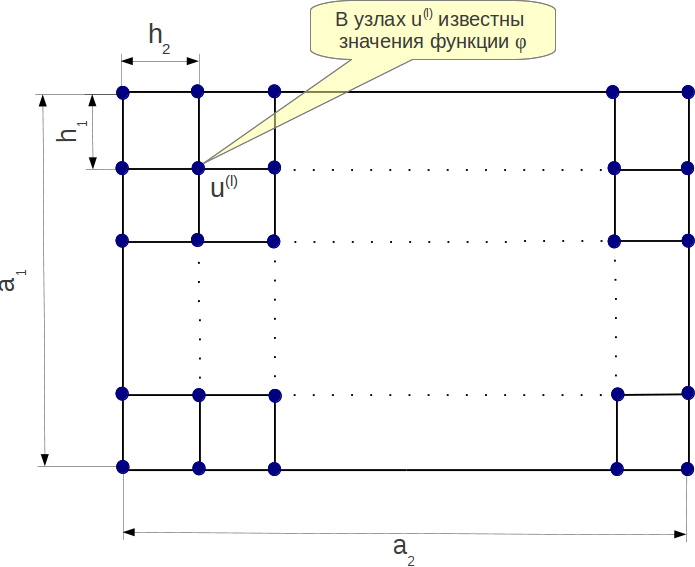
\includegraphics{net_2D}
  \caption{Постановка задачи}
  \label{fig:net_common}
\end{figure}
%\FloatBarrier


%%% Local Variables: 
%%% mode: latex
%%% TeX-master: "paper_func_recv"
%%% End: 



% -*- mode: LaTeX; mode: TeX-PDF; coding: utf-8  -*-

\label{sec:func_recv}

\subsection*{Алгоритм восстановления данных}

Восстановление значения в произвольном  узле $x$    мелкой сетки %в узле $x$,
$r$ раз непрерывно дифференцируемой функции $\varphi$
выполняется следующим образом: 
\begin{gather}
  \label{eq:recv_common}
  G_h(\varphi, x) = \sum_{k\in  \Delta_{K,r}}
   \varphi(u^{(k)})
   \psi_{h, r+\mathbf{2}^n}(x-u^{(k)}),%\\ \notag \text{где}\ 
 \end{gather}
 где $ \Delta_{K,r}=\left[-\lfloor{(r+1)/2}\rfloor:
   K-\mathbf{1}^n+\lfloor{(r+1)/2}\rfloor\right]$.  %\cap\mathbb{Z}_+^n

% <!? а тут тоже надо $\mathbf{1}^n)$ и  $\mathbf{2}^n$ !?>

Из формулы~\eqref{eq:recv_common} следует, что для вычислений
могут быть нужны дополнительные
узлы по краям исходной сетки.
Способы выбора значений в этих узлах зависят
от специфики задачи для которой применяется формула~\eqref{eq:recv_common}  
и в данной работе не рассматриваются.


%%%%%%%%%%%%%%%%%%%%%%%%%%%%%%%%%%%%%%%%%%%%%%%%%%%%%%%%%%%%%%%%%
\subsection*{Схема вычислений}


Введём  следующие обозначения.
\begin{itemize}

\item
  $F$  --- массив  известных значений функции $\varphi$
  в узлах крупной сетки;

\item
  $G_r$ --- массив
  значений аппроксимирующей функции в узлах мелкой сетки,
  вычисленных по формуле~\eqref{eq:recv_common};

\item
  $\Psi_{\rho}$ --- массив  значений ядер В. А. Стеклова порядка $\rho$.

\end{itemize}

%Учитывая финитность и симметрию ядер В. А. Стеклова
%в массиве $\Psi_{2}$ нужно хранить $N^*$
%значений ядер $\psi_{2}$;
%%на одном интервале крупной сетки;
%в массиве $\Psi_{4}$ нужно хранить $2N^*$
%значений ядер $\psi_{4}$.
%на двух смежных интервалах крупной сетки.

Учитывая финитность и симметрию ядер В. А. Стеклова
в массиве $\Psi_{r}$ достаточно хранить $\overline{N(r/\mathbf{2}^n + \mathbf{1}^n) +\mathbf{1}^n}$
значений.

% \emph{Сюда можно вставить рисунок 2D ядра 2го порядка для наглядности.
% Выделить ту четвертинку, которую храним.}
Пример ядра порядка 4 на рисунке, $N=4$.

\begin{figure}[h!]
  \centering
  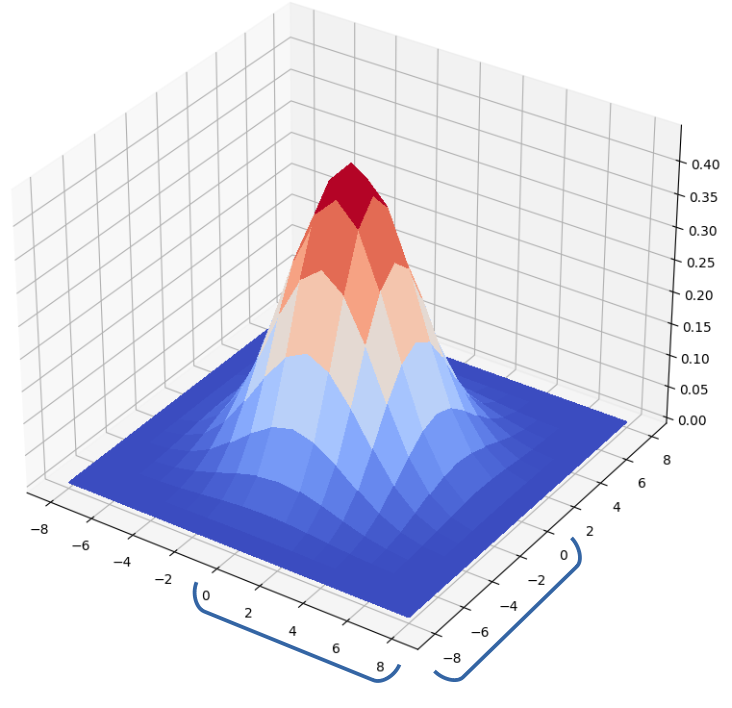
\includegraphics[width=\textwidth
   % ,height
  ]{kern_4_4} 
  \caption{Ядро 4го порядка}
  \label{fig:reg_net}
\end{figure}
\FloatBarrier




Далее приведены выражения для формирования
элементов искомых значений в узлах мелкой сетки,
где $n$ -- количество координат (размерность задачи).

%\emph{Итоговая формула, м.б. от массивов вернуться к функциям?}

\begin{equation}
  \label{eq:nd}
  \begin{split}
    G_r[m] &= 
    \sum_{i \in  [\mathbf{0}^n:r/\mathbf{2}^n + \mathbf{1}^n]} 
        F \left[ \left \lfloor {m}/{N} \right \rfloor - i\right]
      \Psi_{r+\mathbf{2}^n}[iN + m\bmod N] 
       + \\
    &  +
      F \left[\left\lfloor m/N \right \rfloor + (i+\mathbf{1}^n)  \right]
      \Psi_{r+\mathbf{2}^n}[(i+\mathbf{1}^n)N - m \bmod N]
  \end{split}
\end{equation}

На вычисления по формуле~\eqref{eq:nd} требуется

в двумерном случае (2 - операции * и +, 4 части)

$2 * 4 * \overline{(r/\mathbf{2}^n+\mathbf{1}^n) M}.$

в общем случае (2 - операции * и +, $2^n$ частей)

$2 * 2^n * \overline{(r/\mathbf{2}^n+\mathbf{1}^n) M}.$

арифметических операций.

%+(n-1) сложений --- потому что надо сложить результаты по координатам
%А именно для вычисления на одну точку мелкой сетки по каждой координате (2*((r_j+2)-1)) операций:
%(r_j+2) умножение
%и на одно сложение меньше

%По одной координате выражение имеет вид:
% Если $A$ --- $n$-мерный массив, то $[A[i_j]]_j$ означает срез по $j$-й координате, т.~е.
% $A[i_1,\ldots,i_{j-1},i_j,i_{j+1},\ldots,j_n]$, где $i_l$ фиксированы при $l\neq j$.

% \begin{equation}
%   \label{eq:1d}
%   \begin{split}
%     [G_r[m_j]]_{j} &= 
%     \sum_{i = 0}^{r_j/2 +1}
%     \left[
%         F \left[ \left \lfloor {m_j}/{N_j^*} \right \rfloor - i\right]
%     \right]_{j}
%     \left[
%       \Psi_{r+\mathbf{2}^n}[iN_j^* + m_j\bmod N_j^*] 
%     \right]_{j}
%        + \\
%     &  +
%     \left[
%       F \left[\left\lfloor {m_j}/{N_j^*} \right \rfloor + (i+1) \right]
%     \right]_{j}
%     \left[
%       \Psi_{r+\mathbf{2}^n}[(i+1)N_j^* - m_j \bmod N_j^*]
%     \right]_{j}
%   \end{split}
% \end{equation}

\begin{comment}
\emph{Двумерный случай:}

\begin{equation*}
  \begin{split}
    G_r[m_1,m_2] &= 
    \sum_{i_1 = 0}^{r_1/2 +1} \sum_{i_2 = 0}^{r_2/2 +1}
        F \left[ \left \lfloor {m_1}/{N_1} \right \rfloor - i_1, \left \lfloor {m_2}/{N_2} \right \rfloor - i_2\right]
      \Psi_{r_1+2,r_2+2}[i_1N_1 + m_1\bmod N_1,i_2N_2 + m_2\bmod N_2] 
       + \\
    &  +
      F \left[\left\lfloor {m_1}/{N_1} \right \rfloor + (i_1+1), \left\lfloor {m_2}/{N_2} \right \rfloor + (i_2+1)  \right]
      \Psi_{r_1+2,r_2+2}[(i_1+1)N_1 - m_1 \bmod N_1,(i_2+1)N_2 - m_2 \bmod N_2]
  \end{split}
\end{equation*}
  
\end{comment}


Иллюстрация при $r=2$ суммирования по одной координате на рисунке.
\begin{figure}[h!]
  \centering
  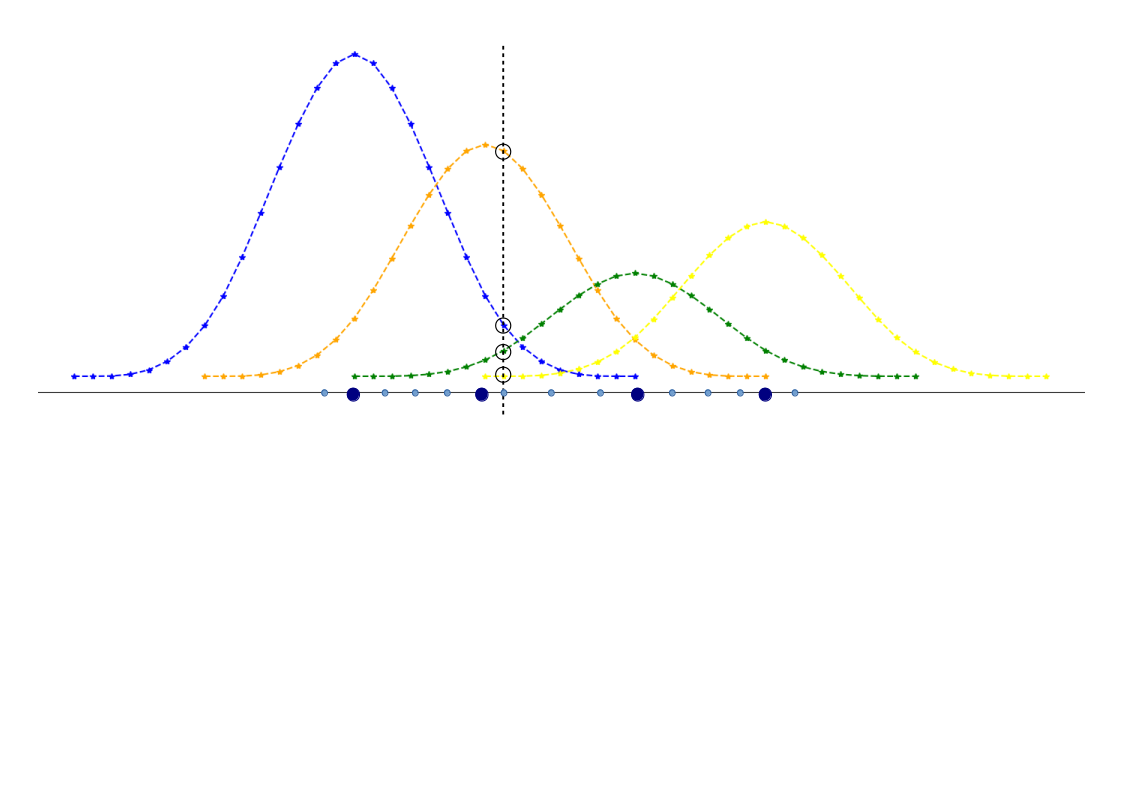
\includegraphics[width=\textwidth,
  %  height=7cm
  ]{multi_kern} 
  \caption{пример для одной координаты}
  \label{fig:reg_net}
\end{figure}
\FloatBarrier



% Заметка про этапы индексации.
% \emph{Можно как=то учесть в обозначениях}
% \begin{enumerate}
% \item
%   Лоцировать ячейку в которой находится искомая точка мелкой сетки.
%   Операция $\left \lfloor \frac{m_j}{N_j^*} \right \rfloor$.

% \item
%   Отобразить индекс в координатах всей мелкой сетки на координаты в ячейке.
%   Операция $m_j \bmod N_j^*$.
% \end{enumerate}
  


%%
\begin{comment}
\begin{itemize}

  \item
Для восстановления данных без сглаживания искомые 
значения в узлах мелкой сетки формируются следующим образом: 
\begin{equation}
  \label{eq:recv_r0}
  \begin{split}
  G_0(m) &=
  F \left( \left \lfloor \frac{m}{N} \right \rfloor \right)\Psi_{2}(m\bmod N) +{}\\
 &+ F \left( \left \lfloor \frac{m}{N} \right \rfloor + 1 \right)\Psi_{2}(N - m \bmod N),
  \end{split}
\end{equation}
где $m = 0, \ldots, M-1$.

Количество арифметических операций при вычислениях непосредственно по формуле~\eqref{eq:recv_r0}
равно $3M$.
%Вычисления по формуле~\eqref{eq:recv_r0} далее будем обозначать алгоритм А1.

\item
%А при $r = 2$ формула~\eqref{eq:recv_common} 
%представляется следующим образом.
Выражение для восстановления данных со сглаживанием имеет вид:
\begin{equation}
  \label{eq:recv_r2}
\begin{split}
  G_2(m) &=  F \left(\left \lfloor \frac{m}{N} \right \rfloor - 1 \right)
              \Psi_{4}(N + m \bmod N)   + {}\\
              &+ F \left (\left \lfloor \frac{m}{N} \right \rfloor \right)
              \Psi_{4}(m \bmod N) +{}\\
              &+ F \left( \left \lfloor \frac{m}{N} \right \rfloor
              + 1 \right)\Psi_{4}(N - m \bmod N)  + {}\\
              &+ F \left(\left \lfloor \frac{m}{N} \right \rfloor + 2 \right)
              \Psi_{4}(2N - m \bmod N),
\end{split}
\end{equation}
где $m = 0, \ldots, M-1$.

Количество арифметических операций при вычислениях непосредственно по формуле~\eqref{eq:recv_r2}
равно $7M$.
%Вычисления по формуле~\eqref{eq:recv_r2} далее будем обозначать алгоритм А2.

\end{itemize}
\end{comment}


Заметим, 
что в формуле~\eqref{eq:nd} каждое из произведений известного значения в узле крупной сетки
со значениями ядер в узлах мелкой сетки используется несколько раз
при формировании результатов в нескольких соседних
%интервалах
ячейках 
крупной сетки. 
С учётом этого факта,
предложена следующая двухэтапная вычислительная схема.
\begin{enumerate}
\item
  %Вычисление произведений значений ядер в узлах мелкой сетки
  %для каждого узла крупной сетки.
  Вычисление для $k$-го ($k \in [0:K-\mathbf{1}^n]$)
  известного значения функции 
  элементов массива произведений
  $\Pi_r[k,l] = F[k]\Psi_{r+\mathbf{2}^n}[l]$,
  ($l \in [0:r(N-\mathbf{1}^n)/2]$).

  Выполняется $\overline{K (N(r/\mathbf{2}^n + \mathbf{1}^n) +\mathbf{1}^n)}$ умножений.
  %$\prod_{i=1}^n K_i(r_iN_i)/2^n$ 
  

\item
  Выбор и суммирование полученных на предыдущем шаге произведений
  для формирования результирующих значений в узлах мелкой сетки
  следующим образом 
\begin{equation}
  \label{eq:nd}
  \begin{split}
    G_r[m] &= 
    \sum_{i \in  [\mathbf{0}^n:r/\mathbf{2}^n + \mathbf{1}^n]} 
        \Pi_r \left[ \left \lfloor {m}/{N} \right \rfloor - i\right, iN + m\bmod N] 
       + \\
    &  +
      \Pi_r\left[\left\lfloor m/N \right \rfloor + (i+\mathbf{1}^n)  \right, (i+\mathbf{1}^n)N - m \bmod N]. 
  \end{split}
\end{equation}

%\emph {в общем случае (2 - операции * и +, 2^n частей) }
%$2 * 2^n * \overline{(r/2+1) M}.$

  Выполняется $2^n * \overline{(r^n/\mathbf{2}^n+\mathbf{1}^n) M}$ сложений.


  %Выполняется $r^2M$ сложений.
  %$M$ сложений в первом варианте и
  %$3M$ сложений --- во втором.
\end{enumerate}

Всего на вычисления по данной схеме требуется

$\overline{K (N(r/\mathbf{2}^n + \mathbf{1}^n) +\mathbf{1}^n)} + 2^n * \overline{(r/\mathbf{2}^n+\mathbf{1}^n) M}$
арифметических операций
вместо

$2^n * \overline{(r/2+\mathbf{1}^n) M} + 2^n * \overline{(r/2+\mathbf{1}^n) M}.$

т.е. сложений одинаковое количество, а умножений

$\overline{K (N(r/\mathbf{2}^n + \mathbf{1}^n) +\mathbf{1}^n)}$

что должно оказаться меньше, чем $2^n * \overline{(r/2+\mathbf{1}^n) M}$.

По порядку значений $KN = M$, тогда выигрыш (примерно) в $2^n$ раз в умножениях. 

%При такой схеме вычислений общее количество арифметических операций
%для восстановления данных без сглаживания
%составляет $2KN + 2K - N$ (что меньше, чем $3M = 3NK + 3K - 3N$)
%и $5KN + 5K - 3N$ (что меньше, чем $7M = 7NK + 7K - 7N$) для
%восстановления данных со сглаживанием.

%Задача восстановления данных в узлах мелкой сетки
%рассматривается как одна стадия конвейера в модели БСКП.
%ВПД этой стадии является массив $F$ размером $K$,
%содержащий известные
%значения в узлах крупной сетки.
%Обработка ВПД  %восстановления значений в узлах мелкой сетки
%состоит из двух вычислительных процедур,
%соответствующих перечисленным выше этапам.


Иллюстрация вычислительной схемы на рисунке.
\begin{figure}[h!]
  \centering
  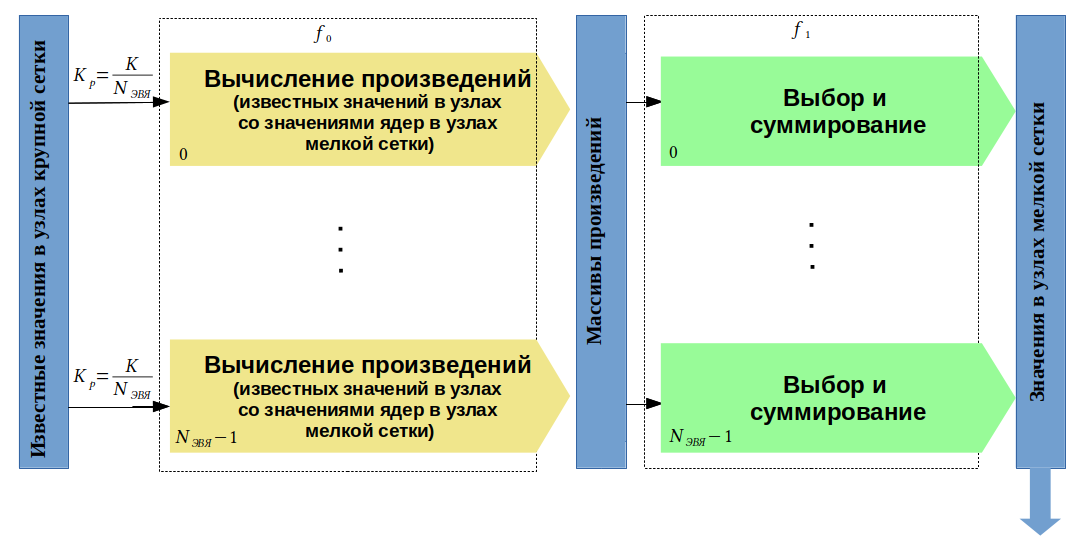
\includegraphics[width=\textwidth,height=7cm]{comp_scheme_steps} 
  \caption{Двухэтапная вычислительная схема}
  \label{fig:reg_net}
\end{figure}
\FloatBarrier


%%%%%%%%%%%%
%-->
%%%%%%%%%%%
\begin{comment}
\subsection*{Параллельные алгоритмы}
Алгоритмы восстановления данных без сглаживания и со сглаживанием
обладают параллелизмом по данным. 
Пусть данная стадия выполняется на ВВЭ состоящем из  $P$ ЭЦСП.
%Значения в узлах крупной сетки
%распределены между всеми ЭЦСП равномерно и размещены в их глобальной памяти.

Рассмотрим вариант равномерного размещения значений в узлах крупной сетки при условии, что
между вычислительными элементами на обоих уровнях модели БСКП
(т.~е. как между ЭЦСП, так и между ЭВЯ) предполагается обмен данными.
Тогда на $p$-м ЭЦСП ($p = 0, \ldots, P-1$)
обрабатывается $K_p = K/P$ узлов, $K_p < GMem$.
Каждый ЭЦСП 
параллельно с остальными обрабатывает свою часть
крупной сетки из $K_p$ узлов и
формирует часть мелкой сетки размером $M_p = N(K_p-1) + K_p$.
Эти узлы, в свою очередь, 
%распределены,
разбиты 
на ЭПД для вычислений на ЭВЯ.
Размер каждого ЭПД $K_p^j = K_p/N_\text{ЭВЯ}$, где $j = 0, \ldots, N_{\text{ЭВЯ}}-1$.
Здесь, для простоты изложения, считаем, что $K_p^j < {LMem}/{2}$,
$K_p$ кратно $N_{\text{ЭВЯ}}$, а $K$ кратно $P$.
%Если эти условия не выполняются, то потребуется обработка дополнительных ЭПД. 

%При таком размещении исходных узлов 
На втором этапе вычислительной схемы в формировании узлов мелкой сетки
на крайних интервалах каждой из частей крупной сетки  
участвуют произведения, которые оказались вычисленными в соседних
вычислительных элементах. % (ЭЦСП или ЭВЯ).
%Поэтому требуется обмен данными.
В случае восстановления данных без сглаживания
каждый вычислительный элемент должен получить дополнительные $N$ значений,
со сглаживанием --- дополнительные $4N$ значений.

Если обмен данными между вычислительными элементами на каком-либо из уровней модели БСКП
исключается,  
то необходимо дублировать данные в крайних узлах частей крупной сетки в соседних
вычислительных элементах.
Для алгоритма без сглаживания в каждом вычислительном элементе размещается $K_p+1$ узлов 
крупной сетки и вычисляется на $N$ больше произведений,
а для алгоритма со сглаживанием --- по $K_p + 3$ узла
и вычисляется на $4N$ произведений больше.


Предложенный подход к распараллеливанию по данным 
эффективен, если на одном ЭЦСП обрабатывается %(без учёта дублирования)
$K_p \ge 2 N_{\text{ЭВЯ}}$ узлов крупной сетки для алгоритма без сглаживания и
$K_p \ge 4 N_{\text{ЭВЯ}}$ узлов для алгоритма co сглаживанием.
Следовательно, границы масштабируемости параллельных алгоритмов восстановления данных 
определются следующими неравенствами:
$P \le \left \lfloor \frac{K}{2N_{\text{ЭВЯ}}} \right \rfloor$ для алгоритма 
без сглаживания и 
$P \le \left \lfloor \frac{K}{4N_{\text{ЭВЯ}}} \right \rfloor$ для
алгоритма со сглаживанием.
%сетки значительно
%больше количества вычислительных элементов и
%выражается следующим
%соотношении размера крупной сетки и количества вычислительных элементов:
%$K \ge 4P$.

%\emph{Тут Можно кол-во операций в табличке представить!}
В таблице~\ref{tab:common_compl} приведены
выражения вычислительной сложности $W$,
коммуникационной сложности $H$ и
количества барьерных синхронизаций $S$,
необходимых для 
трёх вариантов 
параллельных вычислительных алгоритмов
восстановления значений в узлах мелкой сетки %без сглаживания
по формуле~\eqref{eq:recv_r0} и
%со сглаживанием
по формуле~\eqref{eq:recv_r2}.
%на P вычислительных элементах 

\begin{table}[h!] 
  \begin{tabular}{|p{0.17\textwidth}|p{0.38\textwidth}|p{0.38\textwidth}|}
    %%
    \hline
    & без сглаживания & со сглаживанием \\
    \hline
    Без применения двухэтапной вычислительной схемы  &
    %    $$W = \frac{3(NK + K)}{P} - 3N$$
    $$W = 3K_{p}(N + 1) - 3N$$
    $$H = 0; \ S = 0$$ & 
    %    $$W = \frac{7(NK + K)}{P} - 7N$$
    $$W = 7K_{p}(N + 1) - 7N$$
    $$H = 0; \ S = 0$$ 
    \\
    \hline
    По двухэтапной вычислительной схеме с обменами &
    %    $$W = \frac{2(NK + K)}{P} - N$$
    $$W = 2K_{p}(N + 1) - N$$
    $$H = N+1; \ S = 1$$ & 
    %    $$W = \frac{5(NK + K)}{P} - 3N$$
    $$W = 5K_p(N + 1) - 3N$$
    $$H = 4(N+1); \ S = 1$$ 
    \\
    \hline
    По двухэтапной вычислительной схеме без обменов &
    %    $$W = \frac{2(NK + K)}{P} + 1$$
    $$W = 2K_{p}(N + 1) + 1$$
    $$H = 0; \ S = 1$$ & 
    %    $$W = \frac{5(NK + K)}{P} + 3N + 6$$
    $$W = 5K_{p}(N + 1) + N + 4$$
    $$H = 0; \ S = 1$$ 
    \\
    \hline
  \end{tabular}
  \caption {Сводная таблица со сложностями параллельных алгоритмов
    восстановления значений в узлах мелкой сетки}
  \label{tab:common_compl}
\end{table}
%\FloatBarrier 

Из таблицы~\ref{tab:common_compl} видно, что  
алгоритмы с передачей данных и без передачи данных
имеют одинаковую сложность, если пропускная способность, 
с которой вычислительные элементы могут обмениваться данными, равна единице.
Если эта пропускная способность меньше единицы,
то эффективнее алгоритм с передачей данных, а 
если больше, то выгоднее посчитать лишние произведения и данные не передавать.
%Но выбор между алгоритмом с передачей данных и алгоритмом с дополнительными вычислениями,
%но без передачи в конечном итоге зависит от архитектурных особенностей целевой системы.
%Например, даже при условии низкой пропускной способности коммуникационной среды
%если система поддерживает DMA (т. е. предоставляет возможность передачи данных на фоне вычислений),
%то велика вероятность, что эффективнее окажется вариант алгоритма с передачей данных.
\end{comment}


\begin{comment}
\subsection*{Описание программной реализации}

Алгоритмы восстановления данных без сглаживания и со сглаживанием
реализованы в виде библиотеки функций на языке Си.
%Далее рассматриваются подробно действия на каждом из супершагов
%для алгоритмов восстановлений со сглаживанием и без сглаживания.
%При этом именно такая последовательность супершагов в алгоритме со сглаживанием
%позволяет эффективно использовать память.
Каждый из них состоит из двух вычислительных процедур. 
Рассмотрим подробнее реализованные для этих алгоритмов вычислительные процедуры.

\subsubsection{Алгоритм А1 для восстановления данных в узлах мелкой сетки без сглаживания}
%Параллельный алгоритм для 
%вычисления значений в узлах мелкой сетки
%по формуле~\eqref{eq:recv_r0} (т.~е. без сглаживания)
%в терминах модели BSP состоит из двух <<супершагов>>.

\begin{enumerate}
\item
  Каждый вычислительный элемент выполняет следующие действия.
  
  \begin{itemize}
  \item
    Формирует $N$ элементов массива произведений
    $\Pi_2$  
    для первого узла 
    части крупной сетки, обрабатываемой на текущем вычислительном элементе.
%    со значениями ядер В. А. Стеклова
%    второго порядка (вычислены на этапе инициализации и хранятся в памяти).
    
  \item
    В случае варианта реализации с обменами:  
    посылает $N$ значений сформированных %для крайнего узла крупной сетки
    произведений другому вычислительному элементу
    (где обрабатывается предыдущая часть крупной сетки).
    
  \item
    В случае варианта реализации без обменов:
    вычисляет $N$ элементов массива произведений
    $\Pi_2$  
    для дополнительного $K_p$-го узла
    части крупной сетки при наличии этого узла. 
    Если обрабатываемая часть сетки %последняя ---b
    содержит узел с номером $K-1$, то 
    формируется <<код отсутствия>>.
  \end{itemize}
  
\item
  Каждый вычислительный элемент выполняет следующие действия.

  \begin{itemize}
  \item
    В случае варианта реализации с обменами:
    принимает $N$ дополнительных значений произведений
    (которые необходимы для формирования
    значений в узлах мелкой сетки на крайнем справа интервале)
    или <<код отсутствия>>,
    если обрабатываемая на вычислительном элементе
    часть сетки %является последней.
    содержит узел с номером $K-1$.
  \item
    В случае варианта реализации без обменов:
    в качестве дополнительных значений используются
    произведения для $K_p$-го узла,
    сформированные текущим вычислительным элементом
    в предыдущей вычислительной процедуре. 
    
  \item
    Независимо формирует оставшиеся $(K_p - 1)N$ произведений 
    и вычисляет попарным суммированием соответствующих произведений
    $K_p N$ значение в узлах мелкой сетки
    при наличии дополнительных данных %от другого вычислительного элемента
    или
    $(K_p-1) N$ значений в случае <<кода отсутствия>>.
  \end{itemize}
\end{enumerate}


\subsubsection{Алгоритм А2 для восстановления данных в узлах мелкой сетки со сглаживанием}
%Параллельный алгоритм для 
%вычисления значений в узлах мелкой сетки со сглаживанием 
%по формуле~\eqref{eq:recv_r2} 
%в терминах модели BSP состоит из двух <<супершагов>>.

\begin{enumerate}
  \item
    Каждый вычислительный элемент выполняет следующие действия.
    \begin{itemize}
    \item
      Формирует %$3(2N + 2) $ значений произведений
      три массива произведений $\Pi_4$ для 
      узлов с номерами 0, 1  и $K_p - 1$ части крупной сетки, обрабатываемой на текущем
      вычислительном элементе. 
%      со значениями
%      ядер В.~А.~Стеклова четвёртого порядка.

    \item
      В случае варианта реализации с обменами: 
      посылает
      $2N$ значений произведений для 0-го узла текущей части крупной сетки и  %$K_p - 2$
      $N$ значений произведений для 1-го узла текущей части крупной сетки %$K_p - 1$ и
      вычислительному элементу, где обрабатывается предыдущая часть крупной сетки, 
      а $N$ значений произведений для последнего узла --- 
      вычислительному элементу, где обрабатывается её следующая часть.

    \item
      В случае варианта реализации без обменов:
      вычисляет $N$ элементов массива произведений
      $\Pi_4(n)$, $n = N, \ldots, 2N-1$, для 
      дополнительного узла слева;
      $2N$ элементов массива произведений
      $\Pi_4(n)$, $n = 0, \ldots, 2N-1$,
      для первого дополнительного узла справа;  
      $N$ элементов массива произведений
      $\Pi_4(n)$, $n = N, \ldots, 2N-1$, 
      для второго дополнительного узла справа.
      В случае отсутствия какого-либо из дополнительных узлов
      вместо соответствующих произведений формируются <<коды отсутствия>>. 
    \end{itemize}
    
  \item
    Каждый вычислительный элемент выполняет следующие действия.
    \begin{itemize}
    \item
      В случае варианта реализации с обменами: 
      принимает $4N$ дополнительных 
      значений произведений
      или <<коды отсутствия>>.
      
    \item
      В случае варианта реализации без обменов:
      вместо принятых значений произведений используются
      произведения для соответствующих дополнительных узлов,
      сформированные текущим вычислительным элементом
      в предыдущей вычислительной процедуре. 

    \item
      Независимо формирует $2N(K_p - 3)$
      оставшихся  произведений
      и суммирует по 4 соответствующих произведения, получая
      $K_p N$ значений в узлах мелкой сетки при наличии
      дополнительных данных справа или  
      %от вычислительного элемента, где обрабатывается следующая часть исходной крупной сетки или
      $(K_p-1) N$ значений --- если часть сетки %является последней.
      содержит узел с номером $K-1$.
    \end{itemize}
\end{enumerate}

 
%\emph{Замечание про <<кольцевой буфер>>.} 
Объединение суммирования с формированием произведений для не крайних
узлов крупной сетки во второй вычислительной процедуре  
позволяет сократить объём памяти, необходимой для хранения
значений произведений. Вместо хранения второго экземпляра мелкой сетки
со всеми значениями произведений можно хранить 
$2 \times N$ или
$4 \times 2N$
произведений соответственно, которые нужны для
вычисления значений в узлах мелкой сетки на
текущем интервале.
Для организации хранения произведений применяется структура данных
<<кольцевой буфер>>.

\end{comment}

%%
%\bibitem {Zhuk}
%Жук~В.~В. Методические указания к курсу <<Теория аппроксимации функций и ее
%приложения>>. Часть 2. С.-Петербургский ун-т. 1993. 41~с.


%%% Local Variables: 
%%% mode: latex
%%% TeX-master: "paper_func_recv"
%%% End: 





% -*- mode: LaTeX; mode: TeX-PDF; coding: utf-8  -*-


\label{sec:OCLprog}


%\subsection*{Основные обозначения}
\subsection*{Описание программы восстановления данных на OCL}


Современные графические процессоры (GPU --- Graphic Processor Unit)
включают в себя большое количество простых 
вычислительных элементов. %поэтому 
Вычислительные системы с GPU в настоящее время находят применение не только для
графического рендеринга, но и для ускорения различного рода
вычислений общего назначения. 
%(известной как GPGPU --- General Purpose GPU).
В силу специфики архитектуры такие системы 
хорошо подходят для эффективной реализации задач,
обладающих массовым параллелизмом.

Выполнена реализация предложенной вычислительной схемы для
двухмерного случая в стандарте Open CL (Open Computational Language)~\cite{doc_OCL}.
Open CL является открытым и широко применяемым стандартов в области вычислений
общего назначения на гетерогенных (неоднородных) системах
(см., например,~\cite{paper_OCL_Komdiv}). %[ссылку или пояснить?].

%% На уровне гетерогенной системы: управляющий процессор -- ускоритель
Модель гетерогенной вычислительной системы в стандарте Open CL 
состоит из управляющего процессора (Host)
и вычислительных ускорителей (Compute Device),
содержащих, в свою очередь 
мультипроцессоры (Compute Unit),
которые включают в себя вычислительные элементы (Processing Element).
Представление вычислительной платформы в Open CL
показано на рисунке~\ref{fig:OCL_platform}.

\begin{figure}[h!]
  \centering
  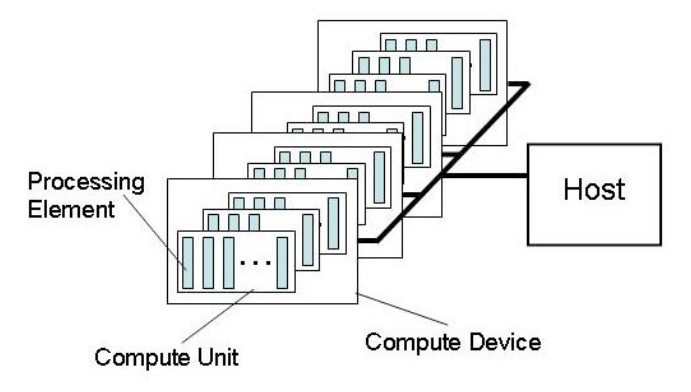
\includegraphics[width=\textwidth,height=7cm]{OCLmodel_platform} 
  \caption{Состав вычислительной платформы в Open CL}
  \label{fig:OCL_platform}
\end{figure}
\FloatBarrier


%% Модель памяти
Иерархия памяти вычислительных ускорителей представляется следующим образом
(см. рисунок~\ref{fig:OCLmodel_mem}).
Всем вычислительным элементам доступна глобальная память (VRAM).
Через VRAM также происходит обмен данными с памятью управляющего процессора (RAM). 
Каждый Compute Unit (мультипроцессор) обладает локальной памятью, к которой имеют доступ
его вычислительные элементы.
Вычислительные элементы имеют внутреннюю (private) память (регистры), доступную только им.

\begin{figure}[h!]
  \centering
  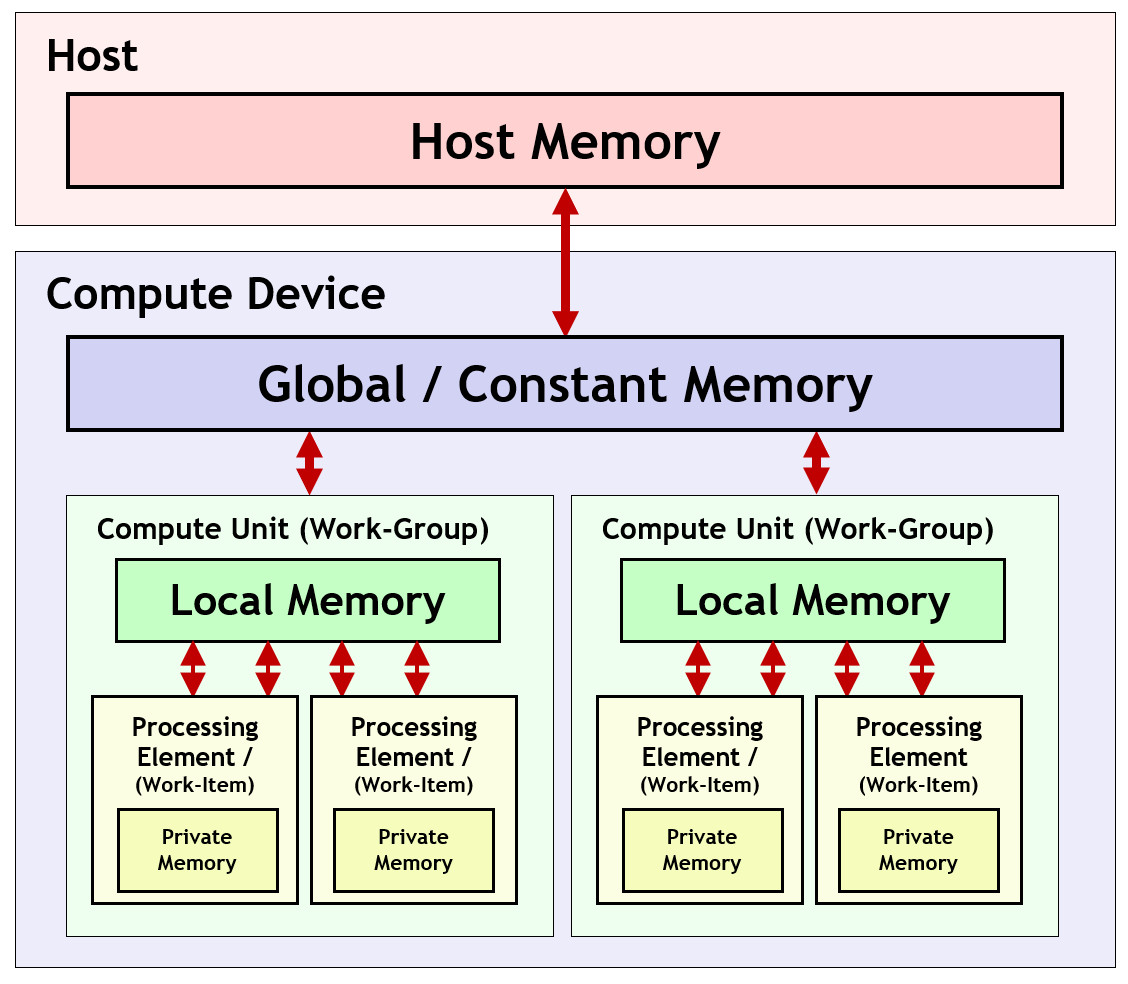
\includegraphics[width=\textwidth,height=7cm]{OCLmodel_mem} 
  \caption{Иерархия памяти вычислительной платформы в Open CL}
  \label{fig:OCL_wg}
\end{figure}
\FloatBarrier

<возможно, будет один обобщённый рисунок>

%Execution of an OpenCL program occurs in two parts: kernels that execute on one or more
%OpenCL devices and a host program that executes on the host. The host program defines the
%context for the kernels and manages their execution.
Исполняемая программа, разработанная в стандарте OpenCL,
содержит:  
вычислительные ядра (kernels), выполняющиеся
параллельно 
в SIMD режиме 
на вычислительных элементах ускорителей
и управляющую программу, которая
определяет контекст и 
управляет запуском вычислительных ядер.

!<Или тут может быть ещё более общий рисунок!>

%% Параллелизм на уровне вычислительных элементов
%Модель параллелизма %программирования
%в OpenCL
%на уровне GPU выражается как SIMT (Single Instruction Multiple Threads) --- терминология CUDA.

%Множество потоков в рамках которых выполняется
%код вычислительных ядер (kernel) выполняется %параллельно
%на множестве вычислительных элементов.

На уровне абстрации модели вычислений в Open CL
вычислительные элементы организованы рабочее пространство:
$n$-мерную решётку,
размером $NDRange$.
Помимо этого вся решётка разбивается на $n_{wg}$-мерные рабочие группы
размером $NDWorkGroup$. 
Для каждого вычислительного элемента в такой модели определены:  
$GlobalID$ %(в общем случае вектор)
--- индекс вычислительного элемента из $[0, NDRange - \mathbf{1}^n]$;
%в пространстве размерности задачи (NDRange).
$LocalID$ --- индекс вычислительного элемента в рабочей группе
из $[0, NDWorkGroup - \mathbf{1}^n]$. 
%пространстве размерности рабочей группы (Work Group).
На рисунке~\ref{fig:OCL_wg} приведён пример
часто встречающегося на практике двумерного рабочего пространства.

\begin{figure}[h!]
  \centering
  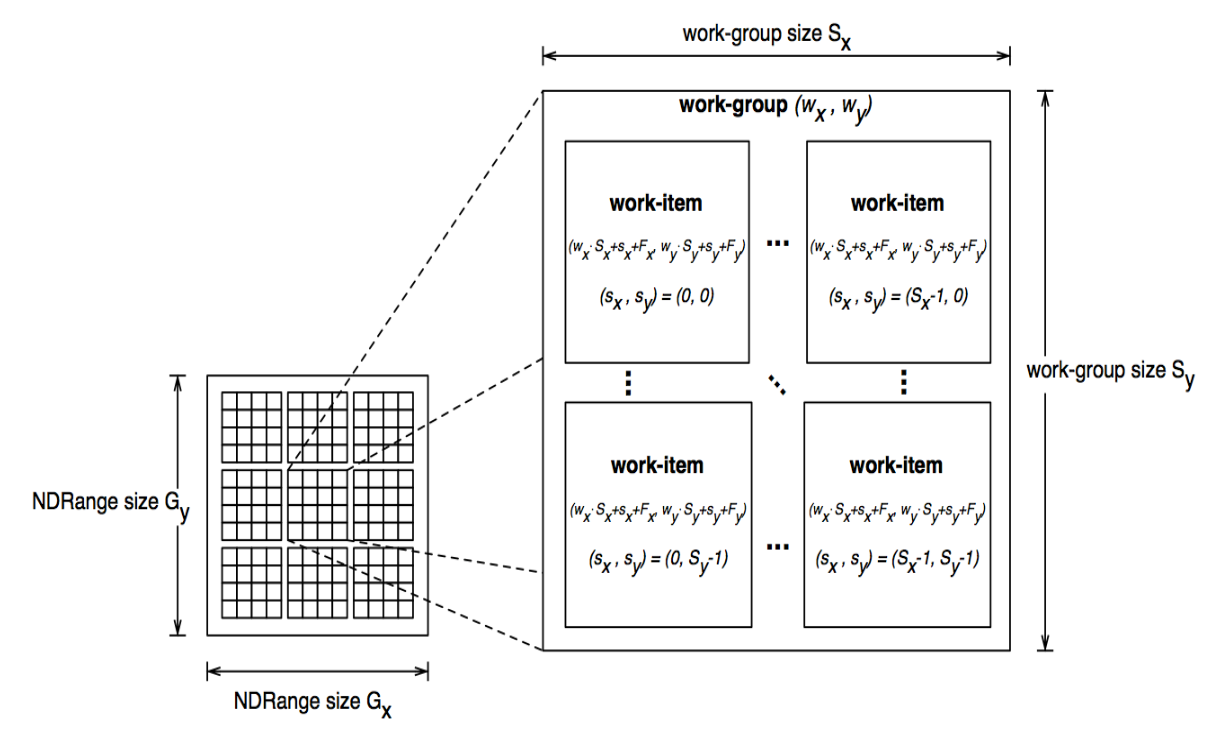
\includegraphics[width=\textwidth,height=7cm]{OCLmodel_wg} 
  \caption{Пример модели рабочего пространства Open CL}
  \label{fig:OCL_wg}
\end{figure}
\FloatBarrier


Из RAM управляющего процессора
в VRAM вычислительного ускорителя
загружаются следующие данные: 
\begin{itemize}
\item
  Массив значений в узлах крупной сетки. %размером $K = K_y*K_x$.
\item
  Массив значений ядра порядка $r$. %, вычисленных в $(r/2)^2$ ячейках мелкой сетки.
  C учётом финитности ядна и его симметричности по
  обом координатам хранить достаточно одну четверть.
  Инициализируется предварительно.
\end{itemize}

Результирующие значения в узлах мелкой сетки выгружаются управляющим процессором
из VRAM по завершению работы вычислительных ядер на ускорителе.

Программная реализация рассмотренного алгоритма в двухмерном случае
включает в себя 2 вычислительных ядра, соответствующие этапам схемы вычислений.
Первое вычислительное ядро выполняется в размерности рабочего пространства $K$,
для второго удобно выбрать размерность $M$.
Далее приведено описание, разработаных вычислительных ядрер.
\begin{itemize}
\item
  {\bf kernel prod}

  Выполняется в каждой точке крупной сетки.
  Каждый вычислительны элемент 
  получает точку крупной сетки
  из VRAM по $globalID$. 
  
  %Размер задачи $K$ (оно же
  %максимальное количество параллельно выполняющихся kernel prod).
  %Размер задачи для этого ядра одномерный (но мб двумерным сделать для наглядности).

  На выходе в VRAM
  формируются массивы произведений в $(r/2)^2$ ячейках мелкой сетки  
  соответствующие каждой точке крупной сетки.
%Выходная структура данных типа map --- для взаимно однозначного соответствия точка -> массив произведений в ячейках.

  
\item
  {\bf kernel sum}

  Суммирует $r$ ближайших по каждой координате к $globalID$ произведений. 
  Выполняется в каждой точке мелкой сетки.
  
  
  Каждый вычислительный элемент записывает свою точку мелкой сетки в
  массив в VRAM по GlobalID
\end{itemize}


%%%%%%%%%%%%%%%%%%%%%%%%%%%%%%%%%%%%%%%%%%%%%%%%%%%%%%%%%%%%%%%%%%%
Результаты работы программной реализации на тестовых данных представлены на графиках~\ref{}.



%%% Local Variables: 
%%% mode: latex
%%% TeX-master: "paper_func_recv"
%%% End: 





\begin{comment}
\subsection*{Заключение}
%\section*{Выводы}


В статье предложена схема вычислений для алгоритмов восстановления данных
без сглаживания и со сглаживанием, которая позволяет сократить
количество арифметических операций, требуемых для их выполнения.
На базе этой схемы построены эффективные параллельные алгоритмы
для класса вычислительных систем, описываемых моделью БСКП.
Произведена теоретическая оценка вычислительной и коммуникационной сложности
предложенных алгоритмов,
выведены зависимости между размерностями задачи и параметрами модели БСКП.

%Рассмотренные алгоритмы применяются для
%повышения частоты дискретизации сигналов
%при программной имитации гидроакустической информации
%линейных антенных решёток.

\end{comment}

% \bibliographystyle{gost705}
% \bibliographystyle{plain}
%\bibliography{bibl}{}

\printbibliography


%\newpage
%\appendix

\end{document}
